In this chapter we will cover the most important families of function of applied algebra. Because of their importance of these families in applications, each section will begin with a motivating real world example and end with a discussion of other applications. Throughout this chapter we will apply all the skills and concepts that appeared previously in this book. 

\par 

Before we begin, let's clarify what we mean by a \it{family of functions}\normalfont. In the symbolic sense, a family of functions is a collection of functions that is defined by a specific algebraic form, often with some set of numbers that appear as parameters in the definition of the family. The function families we will study, and their associated algebraic forms, are the following:
\begin{enumerate}
\item {\bf Linear Functions} - These are functions of the form $y = f(x) = mx + b$, where $m$ and $b$ are constants (numbers).
\item {\bf Quadratic Functions} - These are functions of the form $y = q(x) = ax^2+bx+c$, where $a$, $b$, and $c$ are constants.
\item {\bf Exponential Functions} - These are functions of the form $y = p(x) = ab^{x}$, where $a$ and $b$ are constants.
\item {\bf Power Functions} - These are functions of the form $y = q(x) = ax^{p}$, where $a$ and $p$ are constants.
\end{enumerate}

For each family we will
\begin{enumerate}
\item discuss standard applications, thus leading to an embodied sense of how these functions behave,
\item find formulas for these functions from a set of data,
\item discuss various alternate algebraic forms they may take, with specific reasons to use different algebraic forms,
\item discuss geometric properties of their graphs, and
\item solve algebraic equations involving these functions.
\end{enumerate}

One key thing to keep in mind is that all of the above tasks, and everything we have previously done in this course, are interconnected. Seeing the connections will help you think flexibly about these function families so that you can apply your knowledge assertively in subsequent math and science courses.

\vfill

\pagebreak

\section{Linear Functions}

Linear function make up perhaps the most important class of functions in mathematics. Indeed, the basic premise of Calculus is to approximate more complicated functions with linear ones. However, despite their importance to higher mathematics, they come up in rather simple real world settings.

\begin{eg} Fired Up Pizzeria charges $\$ 9.50$ for a 12 inch pizza with no toppings, then an additional $\$ 1.50$ per topping. Let's consider the function $C$ that takes as an input the number of toppings, $n$, and gives the cost of a pizza, $C(n)$, in dollars. To construct a formula for this function, we first give a table of values for its outputs for several inputs:\\
\begin{center}
\begin{tabular}{c || r | r | r | r | r | r|}
\hline $n$ toppings & $0$ & $1$ & $2$ & $3$ & $4$ \\
\hline $C(n)$ dollars & $9.50$ & $11.00$ & $12.50$ & $14.00$ & $15.50$ \\
\hline
\end{tabular}
\end{center}
The critical thing we notice in this table is that each time the input increases by one unit, an additional $\$ 1.50$ is added to the cost. Hence, the number of times we add $1.50$ to the initial ($n=0$) cost of $\$ 9.50$ is equal to the input $n$. This process of repeated addition is precisely the definition of adding $1.5 n$ to $9.5$, hence we have the formula
\[
C(n) = 9.5 + 1.5 n.
\]
Using the table and/or the formula, we may then graph $C$ (fig. 5.1).

\par

\begin{figure}[h]
\centering
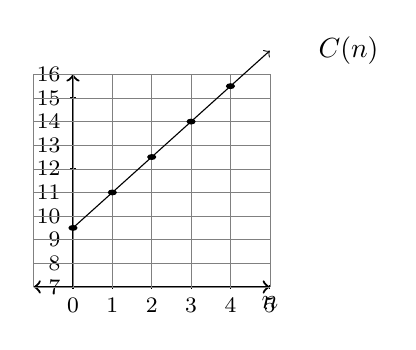
\begin{tikzpicture}[xscale=.5,yscale=.3]
\draw[thick] [<->] (-1,7) -- (5,7);
\draw[thick] [->] (0,7) -- (0,16);
\foreach \x in {0,1,2,3,4,5}\draw[shift={(\x,7)},color=black] (0pt,2pt) -- (0pt,-2pt) node[below] {\footnotesize $\x$};
\foreach \y in {7,8,9,10,11,12,13,14,15,16}\draw[shift={(0,\y)},color=black] (2pt,0pt) -- (-2pt,0pt) node[left] {\footnotesize $\y$};
\draw [help lines] (-1,7) grid (5,16);
\node[align=center,below] at (5,7){$n$};
\node[align=center,above] at (7,16){$C(n)$};
\draw [fill] (0,9.5) circle [radius=0.1];
\draw [fill] (1,11) circle [radius=0.1];
\draw [fill] (2,12.5) circle [radius=0.1];
\draw [fill] (3,14) circle [radius=0.1];
\draw [fill] (4,15.5) circle [radius=0.1];
\draw [domain=0:5] [->] plot (\x, {9.5+1.5*\x});
\end{tikzpicture} 
\caption{The graph of $C(n) = 9.5+1.5n$.}
\end{figure}



In this picture we have plotted the graph between integer values of $n$, even though that may not make sense for this function, so that we can see the defining feature of the graph; it is a straight line. Due to the geometric properties of triangles, we see that the ratio of the change in the output divided by the change input is always equal to $1.5$. This value is called the \it{slope}\ \normalfont of this line.\qed \end{eg} 


\subsection{Intro to Linear Functions}

Using the introductory example given above, we may characterize linear functions as in the following table:\\

\begin{center}
A {\bf Linear Function is $\ldots$}
\begin{tabular}{|p{1.5in} c p{2in}|}
\hline Linear Function & $\longrightarrow$ & A process applied to the input that adds a fixed amount $m$ to the output for each additional unit of input.\\
\ & $\longrightarrow$ & A function of the form $y = f(x) = mx+b$, where $m$ and $b$ are constants.\\
\ & $\longrightarrow$ & A function whose graph is a non-vertical line. \\
\hline
\end{tabular}
\end{center}

Note that when we say that a function is of the form $f(x) = mx+b$, what we really mean is that it can be put into that form throught some algebraic manipulation. The graphical meaning of the parameters $m$ and $b$ are as follows:

\begin{tcolorbox}
{\bf Graphical Meaning of $m$ and $b$}\\
\begin{itemize}
\item $m$ is the slope of the line. That is, given \underline{any}\ \normalfont two points $(x_1,y_1)$ and $(x_2,y_2)$, that lie on the graph of $f$, $m$ is the ratio
\[
m = \frac{y_1-y_2}{x_1-x_2}.
\]
\begin{itemize}
\item If $m>0$, then the graph increases from left to right.
\item If $m<0$, then the graph decreases from left to right.
\item If $m=0$, then the graph is a horizontal line at height $b$.
\item If $|m|$ is larger, the the line is steeper.
\end{itemize}
\item $b$ is the output of $f$ when $x=0$. In other words, it is the $y$-intercept of the graph of $f$.
\end{itemize}
\end{tcolorbox}

\begin{eg} Because a line is uniquely determined by two points, it is possible to find the formula for a linear function whose graph contains a given pair of points (provided the two points do not lie on a vertical line). For instance, suppose we are given that $(1,3)$ and $(3,4)$ are on the graph of $f(x) = mx +b$, and we want to find $m$ and $b$. First we compute the slope:
\[
m = \frac{4-3}{3-1} = \frac{1}{2}.
\]
Then we use the facts that $f$ is of the form $f(x) = \frac{1}{2}x+b$ and one of the two points is on the graph by substituting and solving for $b$:
\begin{eqnarray*}
3 & = & \frac{1}{2}\cdot 1 + b\\
 & \updownarrow & \\
b & = & \frac{5}{2}.
\end{eqnarray*}
Thus $f(x) = \frac{1}{2}x + \frac{5}{2}$. Another way to see how this process works is by noting that $\frac{1}{2}$ is added to the output for every extra unit of input. By starting at $(1,3)$ and subtracting $\frac{1}{2}$ once to get back to when $x=0$, we also get $b=f(0)=\frac{5}{2}$.\qed \end{eg}

\pagebreak

\begin{question} In the last example, we noted that finding the formula for a linear function would not work if the line was vertical. Explain the following:
\begin{enumerate}
\item[a.] You cannot determine the slope of a vertical line from two points on that line.
\item[b.] The equation of a vertical line has the form $x=a$, where $a$ is a number.
\end{enumerate}
\end{question}

\par 

In practical applications, one can often recognize linear functions by noting a rate of change parameter.

\par

\begin{eg} Suppose we wish to find the profit $P$ of selling $q$ widgets. This is the revenue we get from selling the widgets minus the cost of producing them. We sell the widgets for $\$ 35$ a piece, and it costs $\$ 1000$ to set up production, plus $\$ 15$ to make each widget. The units of $\$ /\mbox{widget}$ on the selling price and production cost are both rates of change of the form $(\mbox{function output})/(\mbox{function input})$. This indicates the function is likely a linear function. Going to the formula we get
\[
P = (\mbox{revenue}) - (\mbox{cost}) = 35q - (1000 + 15q).
\]
This simplifies to the linear function
\[
P = 20q - 1000.
\]
Here we see that $\$ 1000$ will be spent no matter how many widgets are sold, and we get a net profit of $\$ 20$ for each widget sold.\qed \end{eg}

\begin{question} A ski shop rents skis for a fixed initial payment of $A$ dollars and a charge of $r$ dollars per day they are used. If a skier pays a total of $A + 6r$ dollars, what is the meaning of the number $6$? Explain your answer as completely as possible.
\end{question}
       
\subsection{Forms of Linear Functions}

The form $y = f(x) = mx + b$ of a linear function is known as \it{slope-intercept form.\ }\normalfont It is a very useful form. A more general (but non-unique) form is known as \it{point-slope form.}\normalfont\\

\begin{tcolorbox}
{\bf Point-Slope Form of a Linear Function}\\
The linear function of slope $m$ passing through the point $(x_0,y_0)$ has the form 
\[
y = f(x) = y_0 + m(x-x_0).
\]
\end{tcolorbox}

In order to understand point-slope form, all you need to do is ask (and answer) the following two questions:
\begin{itemize}
\item Is $f(x) = y_0 + m(x-x_0)$ the formula for a linear function with slope $m$? The answer is yes. All one needs to do is simplify and collect like terms to see that $f(x) = mx + (y_0 - mx_0)$. Thus we can say $b = y_0 - mx_0$.
\item Does the graph of $f(x) = y_0 + m(x-x_0)$ pass through the point $(x_0,y_0)$? Again the answer is yes because $f(x_0) = y_0 + m(x_0-x_0) = y_0$.
\end{itemize}
The graphical difference between point-slope form and slope-intercept form is that slope-intercept form puts on display the $y$-intercept, whereas slope-intercept form displays another point on the graph. Equipped with point-slope form, it is somewhat easier to find a formula for a linear function given two points; all you need to do is compute the slope.

\par 

\begin{question} Use point-slope form to find a formula for the linear function whose graph passes through $(12,7)$ and $(15,89)$. Once you have the formula in point slope form, find the $y$-intercept and write it in slope-intercept form.  
\end{question}

\par

\begin{question} The slope-intercept form of the formula for a linear function is actually equal to the point-slope form for a specific point on the graph. What point is that? 
\end{question}

\par

Since the graphs of linear functions are lines, it makes sense to ask whether the two lines are parallel or perpendicular. To see whether two lines are parallel, they simply must have the same slope. So see whether two lines are perpendicular, consider the following figure:

\begin{figure}[h]
\centering
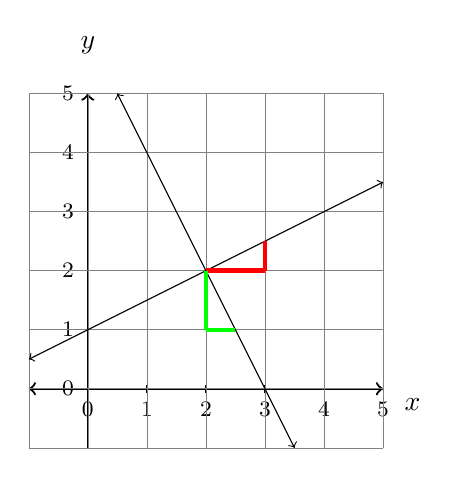
\begin{tikzpicture}[xscale=.75,yscale=.75]
\draw[thick] [<->] (-1,0) -- (5,0);
\draw[thick] [->] (0,-1) -- (0,5);
\foreach \x in {0,1,2,3,4,5}\draw[shift={(\x,0)},color=black] (0pt,2pt) -- (0pt,-2pt) node[below] {\footnotesize $\x$};
\foreach \y in {0,1,2,3,4,5}\draw[shift={(0,\y)},color=black] (2pt,0pt) -- (-2pt,0pt) node[left] {\footnotesize $\y$};
\draw [help lines] (-1,-1) grid (5,5);
\node[align=center,below] at (5.5,0){$x$};
\node[align=center,above] at (0,5.5){$y$};
\draw [domain=-1:5] [<->] plot (\x, {1+0.5*\x});
\draw [domain=.5:3.5] [<->] plot (\x, {6-2*\x});
\draw [ultra thick,red] [-] (2,2) -- (3,2);
\draw [ultra thick,red] [-] (3,2) -- (3,2.5);

\draw [ultra thick,green] [-] (2,2) -- (2,1);
\draw [ultra thick,green] [-] (2,1) -- (2.5,1);

\end{tikzpicture} 
\caption{perpendicular lines}
\end{figure} 

From this (with triangles added to illustrate slope), we see that the magnitude of the change in $y$ for an associated change in $x$ on one graph is the same as the magnitude of the change in $x$ for an associated change in $y$ on the perpendicular graph. Also, the sign of the slope is opposite. Hence the slope of a line perpendicular to a line of slope $m$ is $-\dfrac{1}{m}$.


\begin{question} How can you tell the lines $y = 3x+1$ and $y=3x+17$ never intersect, without doing any algebra? 
\end{question}

\begin{question} Do the graphs of $f(x) = 3x+1$ and $g(x) = 25 + 3(x-8)$ intersect? Why or why not?
\end{question}

\subsection{Applications of Linear Functions}

Linear functions arise in real-world applications involving one variable that changes at a constant rate relative to another. Once the linear function is found, the problems usually boil down to 
\begin{itemize}
\item finding an output for a given input (evaluating),
\item finding the input for a given output (solving a simple equations), or
\item finding when two linear functions are equal (find when graphs intersect).
\end{itemize}

Each of these problems is actually relatively straightforward from an algebraic point of view, given that you have formulas for your functions. The main difficulty is turning the words of the real world into mathematics. 

\par

\begin{eg} As one climbs a mountain, the air temperature decreases by about $3^{\circ}$F for every $1000$ foot increase in elevation. Suppose the temperature is $60^{\circ}$F when at an elevation of $2000$ feet above sea level. Suppose we want the answer to the following questions:
\begin{enumerate}
\item What will the temperature be at an elevation of $14,439$ feet?
\item What should the elevation be to be a ``crisp'' room temperature of $65^{\circ}$F?
\end{enumerate}
\underline{Solutions}\normalfont: Our first task must be to find a formula for temperature as a function of elevation. To achieve this, we first have to name variables (this can be hard at first). Let $T$ be the temperature, in $^{\circ}$F, at an elevation $h$ feet above sea level. The problem describes a rate of change of $-3/1000$ in $^{\circ}$F/ft; this will be the slope of our linear function. This slope can often be seen using the units as the units of slope must be output units divided by input units. The sign is negative because the temperature decreases at this rate as $h$ increases. The problem then describes a point on the graph of this function, $(2000,60)$. Using point-slope form, we have
\[
T = -\frac{3}{1000}(h-2000) + 60.
\]
The answer to part (a) is then obtained by substituting $14,493$ for $h$ to get 
\[
T = -\frac{3}{1000}(14493-2000) + 60\approx 22.521^{\circ}\mbox{F}.
\]
To answer part (b), we need to substitute $65$ for $T$, and solve for $h$:
\begin{eqnarray*}
65 & = & -\frac{3}{1000}(h-2000) + 60\\
 & \updownarrow & \\
h & = & \frac{1000}{3}\approx 333.33\ \mbox{ft}.
\end{eqnarray*}\qed \end{eg}

\par    

\begin{question} Why is the formula for $T$ as a function of $h$ given in the last example more useful to a climber whose elevation is near 2000 feet than to one near sea level? What equivalent formula would be more useful to someone near sea level? Explain.
\end{question}

\par

\begin{question} The ideal gas law says that
\[
PV = nR(T-z),
\]
where $P$ is the pressure of a gas, $V$ is its volume, $T$ is its temperature in $^{\circ}$C, $n$ is the number of moles of gas, $R$ is a constant, and $z$ is the value of absolute zero in $^{\circ}$C. If $n$ and $V$ are constant, like when the gas is in a sealed container, we have a linear function for $P$ as a function of $T$:
\[
P = \frac{nR}{V} (T-z).
\]
\begin{enumerate} 
\item[a.] What is the slope of the graph of $P$ (just in symbols, not the number)?
\item[b.] Suppose we measure $P$ to be $3.5$ when $T = 70$, and $3.602$ when $T = 80$. Find the slope of the graph of $P$ from this data.
\item[c.] Use the data and the value of the slope from part (b) to give an approximate value of $z$. Is this close to the value you may have learned in a science class (or can look up)? 
\end{enumerate} 
\end{question}

\vfill


\pagebreak

\section{Quadratic Functions}

Quadratic functions are probably the simplest non-linear functions to study. The adjective \it{quadratic}\ \normalfont comes from the Latin word for square, \it{quadr$\overline{a}$tus}.\ \normalfont This is because the addition of a term involving $x^2$ comes from measuring areas. Thinking of quadratic functions as ones that measure rectangular areas is what allows us to see that quadratic functions can be used to model positions of objects whose acceleration is constant.  

\subsection{Intro to Quadratic Functions}

A \it{quadratic function}\ \normalfont is one of the form $y = f(x) = ax^2+bx+c$, where $a$, $b$, and $c$ are constants with $a\neq 0$.

\par

\begin{eg} Let us consider the simplest possible quadratic function $f(x) = x^2$. By plotting points, we may construct its graph:

\begin{figure}[h]
\centering
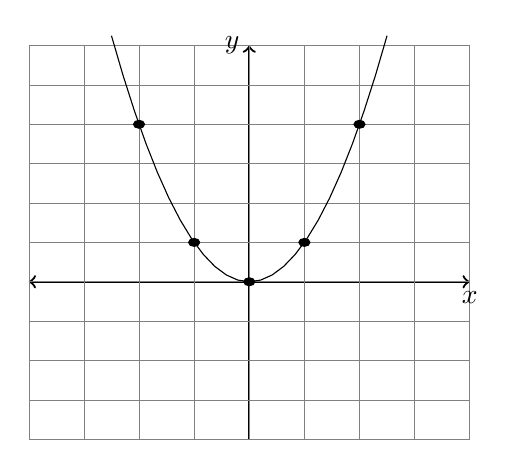
\begin{tikzpicture}[xscale=.7,yscale=.5]
\draw[thick] [<->] (-4,0) -- (4,0);
\draw[thick] [->] (0,-4) -- (0,6);
\draw [help lines] (-4,-4) grid (4,6);
\node[align=center,below] at (4,0){$x$};
\node[align=center,left] at (0,6){$y$};
\draw [fill] (-2,4) circle [radius=0.1];
\draw [fill] (-1,1) circle [radius=0.1];
\draw [fill] (0,0) circle [radius=0.1];
\draw [fill] (2,4) circle [radius=0.1];
\draw [fill] (1,1) circle [radius=0.1];
\draw [domain=-2.5:2.5] plot (\x, {\x*\x});
\end{tikzpicture} 
\caption{The graph of $y=f(x) = x^2$.}
\end{figure} 

There are several observations we can make about the graph, along with connections to the algebraic expression defining this function. 
\begin{itemize}
\item Our first observation is that the outputs of $f(x) = x^2$ are never negative. This is simply due to the fact that the square of any real number is either zero (only when $x=0$) or positive. Not all quadratic functions have non-negative graphs, but the fact that $x^2$ is never negative will be very useful in analyzing other quadratic functions. 
\item Another observation is that the graph is symmetric about the $y$-axis. This is because for any real number $a$, $(-a)^2 = a^2$. Thus the output is the same at $x=a$ as it is for $x=-a$. We will see that the graph of every quadratic function has some vertical axis of symmetry.
\item We see that the graph is \it{concave-up}.\ \normalfont That is, as you move from left to right, the slope between points on the graph is increasing. More precisely, using the input-output table\\
\begin{center}
\begin{tabular}{|c||r|r|r|r|r|r|r|}
\hline $x$ & $-3$ & $-2$ & $-1$ & $0$ & $1$ & $2$ & $3$\\
\hline $f(x)$ & $9$ & $4$ & $1$ & $0$ & $1$ & $4$ & $9$\\
\hline
\end{tabular}
\end{center}

we may construct an table of slopes:

\begin{center}
\begin{tabular}{|p{1in}||p{.5in}|p{.5in}|p{.5in}|p{.5in}|p{.5in}|p{.5in}|}
\hline Points on the Graph & $(-3,9)$ and $(-2,4)$ & $(-2,4)$ and $(-1,1)$ & $(-1,1)$ and $(0,0)$ & $(0,0)$ and $(1,1)$ & $(1,1)$ and $(2,4)$ & $(2,4)$ and $(3,9)$ \\
\hline Slope of Connecting Line & $-5$ & $-3$ & $-1$ & $1$ & $3$ & $5$\\
\hline
\end{tabular}
\end{center}

We see that the slope is increasing. Observing that the slope actually increases by a constant amount for constant steps from left to right is the key to applications of quadratic functions. If the slope were decreasing as we moved from left to right, we would say the graph is \it{concave down}.\normalfont
\end{itemize}

These are the observations we made about $f(x) = x^2$, which has parameters $a=1$, $b=0$, and $c=0$. Throughout this section we will see how the parameters $a$, $b$, and $c$ affect the placement of the maximum or minimum output, the axis of symmetry, and the concavity of the graph of a quadratic function, as well as their practical implications.\qed \end{eg}

\par

\begin{question} In the definition of a quadratic function, it was noted that the parameter $a$ could not be zero. Why would we insist that $a$ be nonzero to define a quadratic function? What do we call a function of the form $f(x) = ax^2+bx+c$ when $a=0$?
\end{question}

\par

Just as the parameters $m$ and $b$ have graphical interpretations for the family of linear functions, the parameters $a$, $b$, and $c$ have graphical  interpretations for quadratic functions. However, because the family of quadratic functions involves three parameters instead of two, they are more complicated.

\par

First let's deal with the parameter $c$. This one is simple; it's just the output of $f(x) = ax^2+bx+c$ when $x=0$. Thus the $y$-intercept of $f(x) = ax^2+bx+c$ is at $(0,c)$. The second easiest parameter to understand is $a$. The sign of $a$ tells use whether the parabola (the graph of a quadratic function is called a \it{parabola}\normalfont) is concave up or concave down. To see this, notice that if $a$ is positive, then for very large values of $x$, $ax^2$ is positive and larger in absolute value than both $bx$ and $c$. This means that the parabola must be opening up. Likewise, if $a$ is negative, then the parabola is concave down. The parameter $b$ is more complicated, and we will leave its exact meaning for the next section.

\par

One of the primary skills associated to any family of functions is solving equations of the form
\[
f(x) = \mbox{a number}.
\]
When $f$ is a quadratic function, we have already discussed one of the most important solution methods: factoring. To solve an equation of the form
\[
ax^2+bx+c = d,
\]
one must just subtract $d$ from both sides, factor, and use the zero factors principle to solve. The $x$-intercepts, or zeros, of a quadratic function can be seen when we write it in \it{factored form}\normalfont:
\[
f(x) = ax^2 + bx+c = a(x-r)(x-s).
\]
In this form $a$ is the same as it is in the expanded form, while $r$ and $s$ are the zeros. Notice that not all quadratic functions can be put into factored form as they may not have any real zeros.

\par
   
\begin{question} When $f(x) = ax^2 + bx + c = a(x-r)(x-s)$, we can use the factors $(x-r)$ and $(x-s)$ to really see what the graph of $f$ looks like, and how $a$ influences it. In what follows, suppose $r$ and $s$ are generic real numbers with $r<s$.
\begin{enumerate}
\item[a.] On a single set of axes graph the lines $y = x-r$ and $y = x-s$. Use this graph to find the values of $x$ where $x-r$ and $x-s$ have the same sign and where they have different signs. Use this do decide when $y=(x-r)(x-s)$ is positive and when it is negative.
\item[b.] Use your answers from part (a) to sketch a graph of $y = (x-r)(x-s)$.
\item[c.] Using your graph from part (b) and reasoning from part (a), explain why the sign of the parameter $a$ tells you whether the graph of $f(x) = a(x-r)(x-s)$ opens up or down.
\end{enumerate}
\end{question}   

\subsection{Forms of Quadratic Functions}

There are three very useful forms of a quadratic function $f(x) = ax^2+bx+c$. The first two are familiar at this point:
\begin{itemize}
\item Standard Form: $f(x) = ax^2+bx+c$.
\item Factored Form: $f(x) = a(x-r)(x-s)$.
\end{itemize}
The third form is new, and is the quadratic analogue of the point-slope form of a linear function.\\

\vspace{.25in}

\begin{tcolorbox}
{\bf Vertex Form of a Quadratic Function}\\
Every quadratic function may be put in the form
\[
y = f(x) = a(x-h)^2+k.
\]
The axis of symmetry of the graph is $x=h$, and the maximum (if $a<0$) or minimum (if $a>0$) output of $f$ is $f(h) = k$. 
\end{tcolorbox} 

The usefulness of vertex form is well illustrated in the following example:

\par

\begin{eg} Let $f(x) = -2(x-3)^2 + 5$. We wish to
\begin{enumerate}
\item[a.] Find the zeros of $f$.
\item[b.] Find the maximum or minimum possible output of $f$. This will tell you the range of $f$.
\item[c.] Sketch the graph of $f$. 
\end{enumerate}
\underline{Solutions:} \normalfont
\begin{enumerate}
\item[a.] Based on prior experience, one may be tempted to expand to standard form and factor. Doing this we obtain the equation
\[
-2x^2+12x-13 = 0.
\]
However, when we try to factor, we see there aren't any ways to do it using only integers. On further reflection, we can see that the vertex form makes it easier to solve, because it breaks a quadratic function into a straightforward process applied to the variable $x$. From the vertex form we can say this function does the following:
\begin{itemize}
\item[\bf S1:] subtract $3$ from $x$
\item[\bf S2:] square {\bf S1}
\item[\bf S3:]  multiply {\bf S2} by  $-2$, and finally
\item[\bf S4:] adds $5$ to {\bf S3}.  
\end{itemize}
The reverse process applied to any output of $f$ will be
\begin{itemize}
\item[\bf undo S4:] subtract $5$ 
\item[\bf undo S3:]and divide by $-2$, then
\item[\bf undo S2:] take the positive or negative square root, and finally
\item[\bf undo S1:] add $3$.
\end{itemize}
Applying this to zero, we get the zeros
\[
x = 3\pm \sqrt{\frac{5}{2}}.
\]
We can apply this to any proposed output, as long as the thing we need to take the square root of is not negative. {\bf Note:} This reverse process does not actually describe an inverse function; the step where the reverse process allows for multiple possibilities prevents this process from defining a function, which must only yield one input for each output.
\item[b.] A slight rearrangement of the vertex form to look like $f(x) = 5-2(x-3)^2$ makes it clear that the range is all $y\leq 5$. Because $(x-3)^2$ is never negative, some quantity is always being subtracted from $5$. The maximum possible output is also clearly $5$, and it occurs when $x=3$. We can also see this from an algebraic expression for the reverse process applied to $y$:
\[
x = 3\pm\sqrt{\frac{y-5}{-2}}.
\]
The possible values of $y$ in this expression are those that make $\frac{y-5}{-2}$ non-negative. Thus we must have $y\leq 5$. 
\item[c.] Plotting the vertex, the $y$-intercept, and a few points to the left and right of the vertex gives us a good graph:

\begin{figure}[h]
\centering
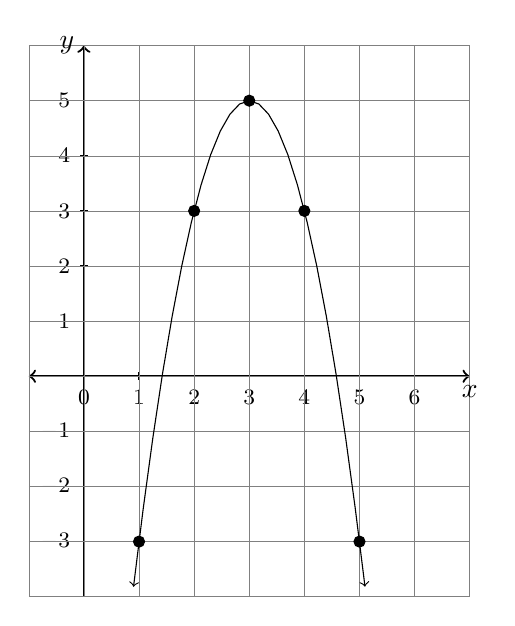
\begin{tikzpicture}[xscale=.7,yscale=.7]
\draw[thick] [<->] (-1,0) -- (7,0);
\draw[thick] [->] (0,-4) -- (0,6);
\foreach \x in {0,1,2,3,4,5,6}\draw[shift={(\x,0)},color=black] (0pt,2pt) -- (0pt,-2pt) node[below] {\footnotesize $\x$};
\foreach \y in {-3,-2,-1,1,2,3,4,5}\draw[shift={(0,\y)},color=black] (2pt,0pt) -- (-2pt,0pt) node[left] {\footnotesize $\y$};
\draw [help lines] (-1,-4) grid (7,6);
\node[align=center,below] at (7,0){$x$};
\node[align=center,left] at (0,6){$y$};
\draw [fill] (3,5) circle [radius=0.1];
\draw [fill] (1,-3) circle [radius=0.1];
\draw [fill] (5,-3) circle [radius=0.1];
\draw [fill] (2,3) circle [radius=0.1];
\draw [fill] (4,3) circle [radius=0.1];
\draw [<->] [domain=.9:5.1] plot (\x, {-2*\x*\x+12*\x-13});
\end{tikzpicture} 
\end{figure}
\end{enumerate}
\qed \end{eg}

\pagebreak

\begin{question} In the last example, we found the zeros of $f(x) = -2(x-3)^2+5$ to be $x=3\pm \sqrt{\frac{5}{2}}$. The zeros are also supposed to appear in the factored form as $r$ and $s$. Expand the right-hand side of the equation and collect like terms to verify that
\[
-2x^2+12x-13 = -2\left(x-\left(3-\sqrt{\frac{5}{2}}\right)\right)\left(x-\left(3+\sqrt{\frac{5}{2}}\right)\right).
\]
\end{question}

\par

One must now ask how we find the vertex form of a given quadratic function, also known as \it{completing the square}.\ \normalfont There are a number of ways to do this. The way we present is very flexible, and may be modified to find useful formulas for many other types of functions. To find the vertex form, simply write down the proposed form with $h$ and $k$, then expand and collect like terms to get a system of equations that you may solve for $h$ and $k$. The following example illustrates this procedure nicely.

\par 

\begin{eg} Find the vertex form of $f(x) = 5x^2-15x+11$ and use it to find the zeros of $f$.\\
\underline{Solution:}\ \normalfont We see $a=5$, thus we must have
\begin{eqnarray*}
5x^2-15x+11 & = & 5(x-h)^2+k\\
\ & = & 5(x^2-2hx+h^2) + k\\
\ & = & 5x^2 - 10hx + 5h^2 + k.
\end{eqnarray*}
Now we match like terms on either side of the equation to obtain the system of equations
\begin{eqnarray*}
-10h & = & -15\ \mbox{(from the $x$ terms)}\\
5h^2 + k& = & 11\ \mbox{(from the constant terms)}
\end{eqnarray*}
Solving this system we have $h = \frac{3}{2}$ and $k = -\frac{1}{4}$. As in the last example, we can solve
\[
5\left(x-\frac{3}{2}\right)^2 - \frac{1}{4} = 0
\]
in a straightforward way to get $x = \frac{3}{2}\pm\frac{1}{\sqrt{20}} = \frac{3}{2}\pm\frac{1}{2\sqrt{5}}$.\qed \end{eg}

One may find the vertex form of a quadratic in full generality in terms of the parameters $a$, $b$, and $c$ ({\bf Do not attempt to memorize this!}):
\[
ax^2+bx+c = a\left(x-\left(\frac{-b}{2a}\right)\right)^2 + \frac{4ac-b^2}{4a^2}.
\]
It is easier to just set up and solve the system of equations, which you'll get faster at with practice, than to commit this to memory. The only reason to write down the general formula for vertex form is to derive the \it{quadratic formula}\ \normalfont for the zeros of a quadratic:
\[
x = \frac{-b\pm\sqrt{b^2-4ac}}{2a}.
\]
Observe that $-\frac{b}{2a}$ is where the vertex is, which is halfway between the zeros. This may be seen as the graphical meaning of the parameter $b$.

\begin{question} Use the quadratic formula to find the zeros of the function in the above example, $f(x) = 5x^2-15x+11$. Simplify your answer to show that it is equivalent to the answer given in the example.
\end{question}

\begin{question} Find the vertex form of the following quadratic functions. Use it to find the maximum or minimum output as well as the zeros of each function, if the zeros exist. Simplify your answers as much as possible, but do not use a calculator.
\begin{enumerate}
\item[a.] $f(x) = 2x^2-4x+1$
\item[b.] $g(x) = 2x^2-4x+5$
\item[c.] $h(x) = 13x^2 -8x + 1$
\end{enumerate} 
\end{question}

The following is a summary of the forms of a quadratic function and what their parameters mean.

\vfill

\pagebreak

\begin{tcolorbox}
{\bf Forms of a Quadratic Function, $f$, and What the Parameters Mean}\\
\begin{itemize}
\item Standard form: $f(x) = ax^2+bx+c$
\begin{itemize}
\item The $y$-intercept of the graph of $f$ is at $(0,c)$.
\item If $a>0$, the graph is an upward opening parabola.
\item If $a<0$, the graph is a downward opening parabola.
\end{itemize}
\item Factored form: $f(x) = a(x-r)(x-s)$.
\begin{itemize}
\item The $x$-intercepts (if they exist) of the graph of $f$ are at $(r,0)$ and $(s,0)$.
\end{itemize}
\item Vertex Form: $f(x) = a(x-h)^2 + k$
\begin{itemize}
\item The vertex of the graph of $f$ is at $(h,k)$.
\item This form is extremely useful for solving equations when factoring proves difficult.
\end{itemize} 
\end{itemize}
\end{tcolorbox}

\begin{eg} Find a formula for the quadratic function whose graph is shown below:

\begin{figure}[h]
\centering
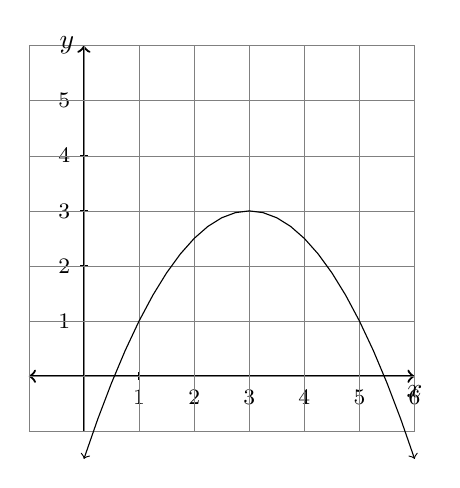
\begin{tikzpicture}[xscale=.7,yscale=.7]
\draw[thick] [<->] (-1,0) -- (6,0);
\draw[thick] [->] (0,-1) -- (0,6);
\foreach \x in {1,2,3,4,5,6}\draw[shift={(\x,0)},color=black] (0pt,2pt) -- (0pt,-2pt) node[below] {\footnotesize $\x$};
\foreach \y in {1,2,3,4,5}\draw[shift={(0,\y)},color=black] (2pt,0pt) -- (-2pt,0pt) node[left] {\footnotesize $\y$};
\draw [help lines] (-1,-1) grid (6,6);
\node[align=center,below] at (6,0){$x$};
\node[align=center,left] at (0,6){$y$};
\draw [<->] [domain=0:6] plot (\x, {-0.5*(\x-3)^2+3});
\end{tikzpicture} 
\end{figure}

\underline{Solution:}\ \normalfont We see that the vertex is at $(3,3)$, hence the quadratic function may be written in the form 
\[
f(x) = a(x-3)^2 + 3.
\]
Using the fact that $(1,1)$ is also on the graph, we have the equation
\[
a(1-3)^2 + 3 = 1.
\]
Solving, we get $a= -\frac{1}{2}$, thus $f(x) = -\frac{1}{2}(x-3)^2 + 3$.\qed \end{eg}

\par

\begin{question} Find a formula for a quadratic function whose graph has $x$-intercepts at $(1,0)$ and $(5,0)$, and $y$-intercept at $(0,7)$.  
\end{question}

\subsection{Applications of Quadratic Functions}

The first application we can see for quadratic functions comes from their original purpose, finding areas. Now that we know how to find the vertex form of a quadratic function, we can find the maximum or minimum possible values of functions that describe area.

\par

\begin{eg} Suppose a farmer wants to fence off a rectangular area with three sides of a rectangle, using a river as the fourth side. She has 100 yards of fence to use and wishes to enclose as large an area as possible. Let $x$ denote the length of the side of the rectangle parallel to the river and $w$ be the length of the side perpendicular to the rive, both measured in yards. Since she has $100$ yards of fence to use, we have the relation
\[
x+2w = 100.
\]
The area is given by $A = xw$. To obtain the area as a function of $x$, we substitute $w=\frac{100-x}{2}$ (from the constraint) for $w$ to get
\[
A(x) = x\left(\frac{100-x}{2}\right) = -\frac{x^2}{2}+50x.
\]
When we find the vertex form of this function we find $h=50$ and $-\frac{h^2}{2} + k = 0$, hence $k = 1250$. Thus
\[
A(x) = -\frac{1}{2}(x-50)^2 + 1250.
\]
This means the maximum area is $1,250$ yd${^2}$, which occurs when $x=50$ and $w = 25$. \qed \end{eg}

\par

\begin{question} How much fence would the farmer in the last problem need if she wanted the maximum possible enclosed area to be $2000$ yd$^2$?
\end{question}

\par

One of the most important applications of quadratic functions comes as a prelude to really doing differential Calculus. The application is modeling the motion of objects with constant acceleration. It was Galileo Galilei who reasoned that all massive objects objects accelerate at the same constant rate when dropped, no matter what the mass is (neglecting air resistance). What we would like to do is construct a function that gives the height of a dropped object $t$ seconds after it was dropped. What type of function should we use? We know that linear functions have a constant rate of change, thus if a linear function is used to describe the position of a moving object, that object's velocity must be constant. This would mean its acceleration must be zero. To model an object whose acceleration is a nonzero constant, we must construct a function whose rate of change changes at a constant rate.    

\par

Let's consider a candidate quadratic function $f(t) = at^2+bt+c$. In order to find the rate of change of the rate of change (let's call this quantity acceleration), we must first find its rate of change for a small change, $\Delta t$, in $t$. To figure this out, let's think flexibly about the terms of $f(t)$ as areas being summed up. The constant term, $c$, can represent a $1\times c$ rectangle, which does not change at all for a $\Delta t$ change in $t$. The term $bt$ can represent a $b\times t$ rectangle. If the side of length $t$ increases by $\Delta t$, the area increases by $b\Delta t$ as in the following figure:\\

\vspace{.1in}

\begin{figure}[h]
\centering
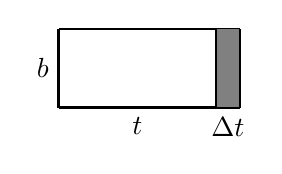
\begin{tikzpicture}
\draw[thick] [-] (0,0) -- (2,0);
\draw[thick] [-] (2,0) -- (2.3,0);
\draw[thick] [-] (0,0) -- (0,1);
\draw[thick] [-] (0,1) -- (2,1);
\draw[thick] [-] (2,1) -- (2.3,1);
\draw[thick] [-] (2,0) -- (2,1);
\draw[thick] [-] (2.3,0) -- (2.3,1);
\draw [fill=gray] (2,0) rectangle (2.3,1);
\node[align=center] at (-.2,.5){$b$};
\node[align=center,below] at (1,0){$t$};
\node[align=center,below] at (2.15,0){$\Delta t$};
\end{tikzpicture}
\end{figure}

The shaded area is the total change in $bt$. Dividing this by $\Delta t$ to make it a rate of change, we find that the rate of change in $bt$ is $b$ (this should not be surprising, $bt$ is linear with slope $b$). Now we will consider the term $at^2$ as the area of a $at\times t$ rectangle. If $t$ changes by $\Delta t$, the total change in $at^2$ is represented by the shaded area in the following figure:

\begin{figure}[h]
\centering
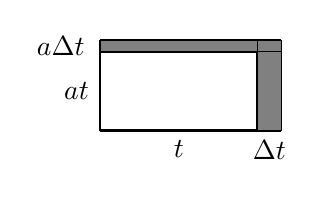
\begin{tikzpicture}
\draw[thick] [-] (0,0) -- (2,0);
\draw[thick] [-] (2,0) -- (2.3,0);
\draw[thick] [-] (0,0) -- (0,1);
\draw[thick] [-] (0,1) -- (2,1);
\draw[thick] [-] (2,1) -- (2.3,1);
\draw[thick] [-] (2,0) -- (2,1);
\draw[thick] [-] (2.3,0) -- (2.3,1);
\draw[thick] [-] (0,1) -- (0,1.15);
\draw[thick] [-] (0,1.15) -- (2,1.15);
\draw[thick] [-] (2,1) -- (2,1.15);
\draw[thick] [-] (2,1.15) -- (2.3,1.15);
\draw[thick] [-] (2.3,1) -- (2.3,1.15);
\draw [fill=gray] (2,0) rectangle (2.3,1);
\draw [fill=gray] (0,1) rectangle (2,1.15);
\draw [fill=gray] (2,1) rectangle (2.3,1.15);
\node[align=center] at (-.3,.5){$at$};
\node[align=center,below] at (1,0){$t$};
\node[align=center,below] at (2.15,0){$\Delta t$};
\node[align=center] at (-.5,1.07){$a\Delta t$};
\end{tikzpicture}
\end{figure}

Thus the total change in $at^2$ for a change in $t$ of $\Delta t$ is given by $2at\Delta t + a(\Delta t)^2$. Dividing by $\Delta t$ to obtain a rate of change, we get $2at + a\Delta t$. Hence the total rate of change in $f(t) = at^2+bt + c$, at a given $t$ value changing by $\Delta t$, is
\[
\mbox{total rate of change} = 2at + a\Delta t + b.
\]
Considering $\Delta t$ to be  ``infinitesimally small'', we find the instantaneous rate of change (velocity) is $2at + b$. This is a linear function with slope $2a$! That means that its rate of change (acceleration) is constant and equal to $2b$. This means we have a new characterization of quadratic functions to go along with their algebraic form:


\begin{center}
A {\bf Quadratic Function is $\ldots$}
\begin{tabular}{|p{1.5in} c p{2in}|}
\hline Linear Function & $\longrightarrow$ & A function of the form $y = f(x) = ax^2+bx+c$, where $a$, $b$, and $c$ are constants.\\
\ & $\longrightarrow$ & A function whose graph is a parabola.\\
\ & $\longrightarrow$ & A function whose second rate of change (acceleration) is constant. \\
\hline
\end{tabular}
\end{center}

{\bf Remark:} The idea of computing instantaneous rates of change is central to Calculus. Re-read this section carefully now, then do it again when you learn about derivatives. 

\begin{eg} Now back to Galileo's problem. He measured the acceleration of an object to be downward at $9.8$ m/s$^2$. Thus, to model the height of a projectile, we should use a quadratic function with leading term $-4.9t^2$. The initial velocity, $v_0$, should be the constant term of the velocity function ($2at+b$ above), so the linear term should be $v_0 t$. The initial height is just the vertical intercept. Hence we have the formula for the height of a object, in meters after $t$ seconds, with initial height $h_0$ and initial velocity $v_0$:
\[
h(t) = -4.9t^2 + v_0t + h_0.
\]
\begin{itemize}
\item To find when it hits the ground, find the larger of its zeros.
\item To find the maximal height, find the vertex.
\end{itemize}

\begin{question} What is the instantaneous rate of change in $f(t) = t^3$? Explain why your answer is correct using the volume of a cube as in Question 2.6. 
\end{question}

\vfill

\section{Exponential Functions}

Exponential functions are common in applications where the rate of change is not described in absolute terms, but in relative terms as a percent rate of change. For instance, suppose we say a population, $P$, is growing at a rate of $50\%$ per year with an initial value of $1000$. This means that to find the population next year, we find the population of the current year, multiply it by $0.5$, and add it to the current population. Then we can construct a table of values, with the input $t$ being measured in years:\\

\vspace{.2in}
\begin{center}
\begin{tabular}{|r || r | r | r | r |}
\hline $t$ & $0$ & $1$ & $2$ & $3$\\
\hline $P$ & $1000$ & $1500$ & $2250$ & $3375$\\
\hline
\end{tabular} 
\end{center}


We can notice that the slope, which is the absolute rate of change, is not constant. Between the points $(0,1000)$ and $(1,1500)$, the slope is $500$. The slope between the points $(1,1500)$ and $(2,2250)$ is $750$. However, if we take the ratio of consecutive outputs, we get a constant:
\[
\frac{1500}{1000} = \frac{2250}{1500} = \frac{3375}{2250}  = 1.5.
\]
What this shows is that each time the input increases by $1$, the output gets multiplied by $1.5$ one more time. Since repeated multiplication is denoted by an exponent, we see that
\[
P = 1000(1.5)^t.
\]
Functions with this basic form are known as exponential functions.


\subsection{Intro to Exponential Functions}

An \it{exponential function}\ \normalfont is a function of the form $f(x) = ab^x$, where $a\neq 0$ and $b>0$. 

\par

\begin{eg} Consider $f(x) = 2(1.5)^x$. We can plot some points to construct a graph of this function.

\begin{figure}[h]
\centering
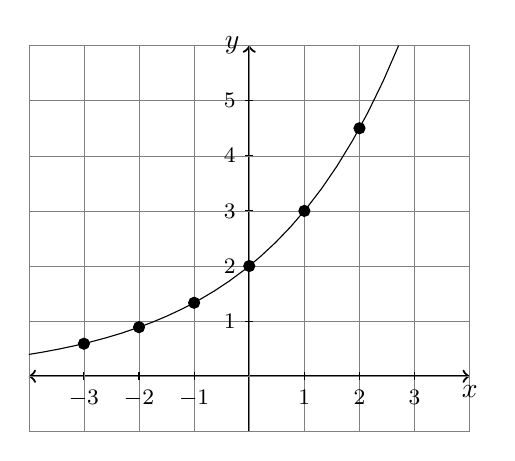
\begin{tikzpicture}[xscale=.7,yscale=.7]
\draw[thick] [<->] (-4,0) -- (4,0);
\draw[thick] [->] (0,-1) -- (0,6);
\draw [help lines] (-4,-1) grid (4,6);
\node[align=center,below] at (4,0){$x$};
\node[align=center,left] at (0,6){$y$};
\foreach \x in {-3,-2,-1,1,2,3,}\draw[shift={(\x,0)},color=black] (0pt,2pt) -- (0pt,-2pt) node[below] {\footnotesize $\x$};
\foreach \y in {1,2,3,4,5}\draw[shift={(0,\y)},color=black] (2pt,0pt) -- (-2pt,0pt) node[left] {\footnotesize $\y$};
\draw [fill] (-2,.89) circle [radius=0.1];
\draw [fill] (-3,.59) circle [radius=0.1];
\draw [fill] (-1,1.333) circle [radius=0.1];
\draw [fill] (0,2) circle [radius=0.1];
\draw [fill] (1,3) circle [radius=0.1];
\draw [fill] (2,4.5) circle [radius=0.1];
\draw [domain=-4:2.71] plot (\x, {2*1.5^(\x)});
\end{tikzpicture} 
\caption{The graph of $y=f(x) = 2(1.5)^x$.}
\end{figure}


We can make several observations about this graph and connect them to the algebraic form of this function. 
\begin{itemize}
\item First, notice that the $y$-intercept is at $(0,2)$. This is due to the fact that $f(0) = 2(1.5)^0$. Since any nonzero number raised to the zero power is $1$, we are just multiplying $2$ by $1$. 
\item We also can notice this function is increasing as you move from left to right. In fact, you can see that each point we plotted is exactly one and a half times higher above the $x$-axis than the point that was plotted one unit to its left. This is because the height is multiplied by $1.5$ each time the input increases by one unit. 
\item If we move from right to left through negative values of $t$, all the outputs are less than $2$ and getting smaller. This isn't a truly different observation than the last one, but it's a different perspective. This comes from the fact that when $t$ is negative, we're really dividing by positive powers of $1.5$. (Review you exponent rules now if you need to.)
\item Finally, we notice that the outputs stay above the $x$-axis. This is because $(1.5)^t$ is always positive, as it represents repeated multiplication of a positive number. If the $2$ in front were replaced by a negative number, then the output would never be positive. Exponential functions never change signs.
\end{itemize}\qed \end{eg}

\begin{question} In the definition of an exponential function, we said that $a$ cannot be zero and $b$ had to be positive. Let's think about why we would make such restrictions.
\begin{enumerate}
\item[a.] If $a=0$, what simpler family of functions does $f(x) = ab^x$ belong to?
\item[b.] If $b$ is negative, what is a value of $x$ that would make $b^{x}$ undefined? (The answer is not zero.)
\end{enumerate} 
\end{question}

\begin{tcolorbox}
{\bf The Meaning of $a$ and $b$ in Exponential Functions}\\
\begin{itemize}
\item $b$ is the growth factor. Each time the input increases by one unit, the output is multiplied by another factor of $b$.
\begin{itemize}
\item If $b>1$, then the graph diverges away from the $x$-axis from left to right and gets arbitrarily close to the $x$-axis as $x\to-\infty$.
\item If $b<1$, then the graph gets arbitrarily close to the $x$-axis as $x\to\infty$, and diverges away from the $x$-axis moving right to left.
\end{itemize}
\item $a$ is the output of $f$ when $x=0$. In other words, it is the $y$-intercept of the graph of $f$.
\end{itemize}
\end{tcolorbox}

\begin{question} The domain of an exponential function is the set of all real numbers. What is the range?  Your answer will  depend of the value of $a$.
\end{question}

\par

As with all function families, when we say that a function has a specific form, we really mean that its defining formula is equivalent to that form. Often it is the case that a function is not presented in a specific form, but algebraic manipulation shows it to be in the specified family.

\par

\begin{eg} Let $f(x) = \dfrac{3(2)^{x+3}}{5^{x-1}}$. This function is not in the form $f(x) = ab^x$, but we may use some exponent rules to put it in that form:
\[
f(x) = \frac{3(2)^{x+3}}{5^{x-1}} = \frac{3\cdot 2^3\cdot 2^{x}}{5^{-1}\cdot 5^{x}} = 120\left(\frac{2}{5}\right)^{x}.
\]
Hence we see $a = 120$ and $b=\frac{2}{5}$. Alternatively, we could use a table of outputs to decide this function is exponential and find its parameters:\\
\begin{center}
\begin{tabular}{|r|| r |r |r|}
\hline $x$ & $0$ & $1$ & $2$ \\
\hline $f(x)$ & $120$ & $48$ & $19.2$\\
\hline
\end{tabular}
\end{center}
The ratios of consecutive values are equal to $b$: $\frac{48}{120} = \frac{19.2}{48} =\frac{2}{5}$. The value at $t=0$ is $a$. \qed \end{eg}

Generally, if you know one of the parameters of an exponential function and a point on its graph, you can solve for the other parameter. In the next section we will go into detail of how to find formulas for exponential functions from two points on the graph, similar to how we did it for linear functions. We will also see possible reasons for alternatives to the standard $ab^x$ form.


\subsection{Forms of Exponential Functions}

Often we would like to find a formula for an exponential function when the initial condition and growth rate are not known. However, we often do know  some information that is somehow equivalent to two points on the graph. To understand some of the useful forms of exponential functions, let's first figure out how to find a formula given two points on the graph.

\par

\begin{eg} Suppose the points $(2,1)$ and $(9,4)$ are on the graph of $y=f(x) = ab^{x}$. We would like to determine $a$ and $b$. To do this, we merely need to set up a system of equations and solve it. Using the input-output pairs, we have
\begin{eqnarray*}
1 & = & ab^{2}\\
4 & = & ab^{9}.
\end{eqnarray*}
Using the first equation, we find $a = \frac{1}{b^2}$, which we can substitute into the second to get
\begin{eqnarray*}
4 & = & \frac{1}{b^2}\cdot b^{9}\\
 & \updownarrow & \\
b^{7} & = & 4 \\
& \updownarrow & \\
b & = & \sqrt[7]{4}.
\end{eqnarray*}
Then we find $a = \frac{1}{(\sqrt[7]{4})^{2}}$. Thus we have $f(x) = \frac{1}{(\sqrt[7]{4})^{2}} (\sqrt[7]{4})^x$. \qed \end{eg}

\par

This process for finding the equation of an exponential function is straightforward, but the final answer does not show the points the graph passes through in a transparent way. Instead, we may write it in the form 
\[
f(x)  = \frac{1}{(\sqrt[7]{4})^{2}} (\sqrt[7]{4})^x = 1\cdot 4^{\frac{x-2}{7}}.
\] 
In this form we can see that $f(2) = 1$ and $f(9) = 4$ quite easily. 

\par

\begin{question} Show the manipulations, using exponent rules, that one must use to put the function from the example into the form shown above.
\end{question}

\par

\begin{question} Let $f(x) = 3\left(\frac{14}{3}\right)^{\frac{x-12}{5}}$. Find two points with integer coordinates that are obviously on the graph of $f$. Explain why they are obvious.
\end{question}

\par

Using the last two questions as motivation, we can introduce the following form of an exponential function:

\begin{tcolorbox}
{\bf Point-Factor-(Time Interval) Form for an Exponential Function}\\
An exponential function $f$ that has the property that $f(x_0) = S$ and grows by a factor of $M$ over each time interval $T$ has the form 
\[
f(x) = S(M)^{\frac{x-x_0}{T}}.
\]
The initial value of this function is $\left(S(M)^{-\frac{x_0}{T}}\right)$ and its growth factor per unit increase in input is $M^{\frac{1}{T}}$. 
\end{tcolorbox}

This particular form of an exponential function may be thought of as analogous to the point-slope form of a linear function. However, because the formula is a bit more complicated, it may be more useful to use it only implicitly, and think about why your answer is right.

\par

\begin{eg} Suppose a quantity $Q= f(t)$ grows exponentially as a function of $t$, where $Q = 3$ when $t=2$, and $Q$ increases by $25\%$ every time $t$ increases by $20$. Find a formula for $Q$ in terms of $t$.

\par

\underline{Solution:}\ \normalfont Since $Q$ grows by $25\%$ each time $t$ increases by $20$, each time $t$ increases by $20$, the initial quantity will be multiplied by $1.25$. This means the exponent of $1.25$ should be divided by $20$. Since the output is $3$ when $t=2$, we can put $t-2$ as the numerator in the exponent. Thus we have
\[
Q = f(t) = 3(1.25)^{\frac{t-2}{20}}.
\]
Now we may ask ourselves whether this behaves in the specified way:
\begin{itemize}
\item Is $f(2) = 3$? Yes, $f(2) = 3(1.25)^{\frac{2-2}{20}} = 3$.
\item Is $Q$ multiplied by an additional factor of $1.25$ each time $t$ increases by $20$. Yes, observe
\begin{eqnarray*}
f(2) & = & 3\\
f(22) & = & 3(1.25)^{\frac{20}{20}} = 3(1.25)\\
f(42) & = & 3(1.25)^{\frac{40}{20}} = 3(1.25)^2\\
\ & \vdots & \\
\end{eqnarray*}
\end{itemize}
Thus we can see that this function behaves in the specified way. \qed \end{eg}

Another form of an exponential function is indicated by the preceding example. Often, in real world applications, exponential functions are described by a constant percent growth rate. 

\begin{tcolorbox}
{\bf Percent Growth Rate Form of an Exponential Function}\\
Every exponential function $f(x) = ab^{x}$ may be written in the form 
\[
f(x) = a(1+r)^{x}.
\]
In this form $r = b-1$ is the percent growth (when multiplied by $100\%$) for each unit increase in $x$.
Note:
\begin{itemize}
\item If $b>1$, then $r>0$. In this case $r$ is just called the growth rate.
\item If $0<b<1$, then $r<0$. In this case $|r|$ is the decay rate.
\end{itemize}
\end{tcolorbox}

\begin{question} In the function $Q=f(t) = 3(1.25)^{\frac{t-2}{20}}$, by what percent does $Q$ grow per unit increase in $t$?
\end{question}


\subsection{Applications of Exponential Functions}

Standard applications of exponential functions are those related to growth and decay. We will introduce these applications now, but investigate them further when we are equipped with logarithms. Logarithms will allow us to solve equations involving exponential functions.

\begin{eg} Suppose a population of bacteria, $P$, in millions starts at $P = 4$ and triples every six hours. Find a formula for $P$ as a function of time $t$, in hours. By what percent does $P$ change each hour?\\
\underline{Solution:} Using the point-factor-time interval idea, we find 
\[
P = 4(3)^{\frac{t}{6}}.
\]
In order to find the growth rate, we must first find the growth factor $b$. This is done by applying exponent rules:
\[
P = 4(\sqrt[6]{3})^{t}.
\]
Hence the growth factor is $b = \sqrt[6]{3}\approx 1.201$. Hence the percent growth rate is about $20.1\%$ per hour.\qed \end{eg}

\begin{question} Cesium-137 is a radioactive isotope formed in nuclear fission. Given that it decays at a rate of $2.27\%$ per year, what equation would you need to solve in order to find its half-life (the time it takes for half of an initial quantity to remain)?
\end{question}


\section{Power Functions}

The last basic family of functions we study will also be a two-parameter family. This is the family of \it{power functions}.\normalfont\ These are functions of the form 
\[
f(x) = kx^{p}.
\]
We call $k$ the \it{coefficient}\ \normalfont of the power function and $p$ the \it{exponent}.\normalfont\ There are no restrictions placed on $k$ and $p$; they can be any constant.

\par

\begin{question} What conditions on $k$ and $p$ would place a power function into one of the other families of functions we have studied (list all possibilities)? Explain.
\end{question}

\par

\begin{question} Are there any values of $k$ and $p$ such that a power function could be called an exponential function? Explain.
\end{question}

\par

While the class of power functions still only has two parameters, we will see they are somewhat more complicated than the families of linear and exponential functions. Power functions can have a much wider array of graphs and may exhibit more complicated domains and ranges than linear or exponential functions. However, much of the complication can be worked out by remembering our rules of arithmetic.

\subsection{Intro to Power Functions}

Consider the following three power functions:

\[
f(x) = x^{4},\ \ g(x) = \frac{1}{x^4},\ \ \mbox{and}\ \ h(x) = x^{\frac{1}{4}}.
\]
Their coefficients are all equal to one. Their exponents are $4$, $-4$, and $\frac{1}{4}$, respectively. The simplest of these to graph is $f$:


\begin{figure}[h]
\centering
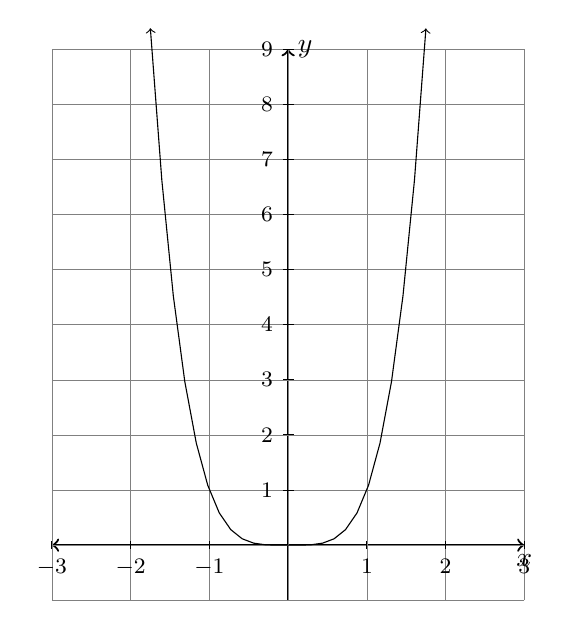
\begin{tikzpicture}[xscale=1,yscale=.7]
\draw[thick] [<->] (-3,0) -- (3,0);
\draw[thick] [->] (0,-1) -- (0,9);
\draw [help lines] (-3,-1) grid (3,9);
\node[align=center,below] at (3,0){$x$};
\node[align=center,right] at (0,9){$y$};
\foreach \x in {-3,-2,-1,1,2,3}\draw[shift={(\x,0)},color=black] (0pt,2pt) -- (0pt,-2pt) node[below] {\footnotesize $\x$};
\foreach \y in {1,2,3,4,5,6,7,8,9}\draw[shift={(0,\y)},color=black] (2pt,0pt) -- (-2pt,0pt) node[left] {\footnotesize $\y$};
\draw [domain=-1.75:1.75] [<->] plot (\x, {(\x)^4});
\end{tikzpicture} 
\caption{The graph of $y=f(x) = x^4$.}
\end{figure}

We see from the graph that $f(x) = x^4$ is similar in shape to $y = x^2$. The outputs are never negative because the exponent is even, and the minimum output is zero. We see that the outputs grow more rapidly than those of $y = x^2$ when $|x|>1$ and decay to zero more rapidly when $|x|<1$. This is simply a result of repeating the multiplication of $x$ by itself four times instead of two. As the exponent grows, this effect is exaggerated. 


\pagebreak

A slightly more complicated graph is that of $g(x)$:


\begin{figure}[h]
\centering
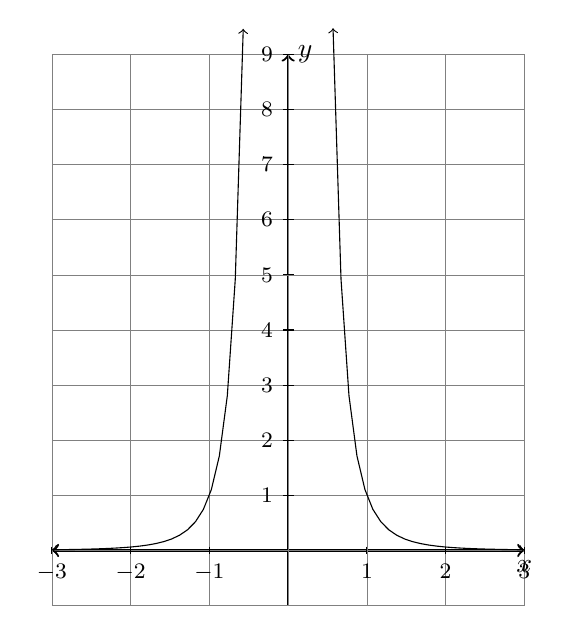
\begin{tikzpicture}[xscale=1,yscale=.7]
\draw[thick] [<->] (-3,0) -- (3,0);
\draw[thick] [->] (0,-1) -- (0,9);
\draw [help lines] (-3,-1) grid (3,9);
\node[align=center,below] at (3,0){$x$};
\node[align=center,right] at (0,9){$y$};
\foreach \x in {-3,-2,-1,1,2,3}\draw[shift={(\x,0)},color=black] (0pt,2pt) -- (0pt,-2pt) node[below] {\footnotesize $\x$};
\foreach \y in {1,2,3,4,5,6,7,8,9}\draw[shift={(0,\y)},color=black] (2pt,0pt) -- (-2pt,0pt) node[left] {\footnotesize $\y$};
\draw [domain=-3:-.57] [<->] plot (\x, {(\x)^(-4)});
\draw [domain=.57:3] [<->] plot (\x, {(\x)^(-4)});
\end{tikzpicture} 
\caption{The graph of $y=g(x) = \frac{1}{x^4}$.}
\end{figure}

In this graph, we never see negative outputs because the exponent is even. However, we also never see zero as an output because a fraction is only zero when its numerator is zero at the same time its denominator is not zero. The most conspicuous behavior of this function is that as $|x|$ gets large, $g(x)\to 0$ and as $|x|$ gets close to zero, $g(x)\to \infty$. This is a simple consequence of arithmetic; if you divide by a large number, the result is small and if you divide by a positive number very close to zero, the result is very large.

\par

Finally, we can graph $h(x) = x^{\frac{1}{4}}$:

\begin{figure}[h]
\centering
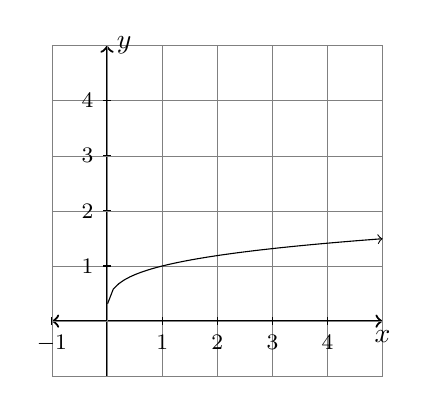
\begin{tikzpicture}[xscale=.7,yscale=.7]
\draw[thick] [<->] (-1,0) -- (5,0);
\draw[thick] [->] (0,-1) -- (0,5);
\draw [help lines] (-1,-1) grid (5,5);
\node[align=center,below] at (5,0){$x$};
\node[align=center,right] at (0,5){$y$};
\foreach \x in {-1,1,2,3,4}\draw[shift={(\x,0)},color=black] (0pt,2pt) -- (0pt,-2pt) node[below] {\footnotesize $\x$};
\foreach \y in {1,2,3,4}\draw[shift={(0,\y)},color=black] (2pt,0pt) -- (-2pt,0pt) node[left] {\footnotesize $\y$};
\draw [domain=.01:5,samples=50] [->] plot (\x, {(\x)^(.25)});
\end{tikzpicture} 
\caption{The graph of $y=g(x) = x^{\frac{1}{4}}$.}
\end{figure}

\pagebreak

In this graph we notice that the domain is only non-negative $x$-values. This is because even roots of negative numbers are not defined. Also, even roots of numbers are defined to be positive, so the range is all $y \geq 0$. The shape of the graph can be seen by noting that if $y=x^{\frac{1}{4}}$, then $x=y^4$. This means that the graph of $y=x^{\frac{1}{4}}$ is that of the positive half of $y=x^{4}$, but reflected across the  line $y=x$.

\begin{question} Sketch graphs of $f(x) = x^{3}$, $g(x) = x^{-3}$, and $h(x) = x^{\frac{1}{3}}$. What is the main difference between these graphs and the graphs given above, and how can you explain the difference in terms of basic arithmetic?
\end{question}

\begin{question} For each of the following conditions on $k$ and $p$, sketch a rough graph of $f(x) = kx^{p}$. Explain why your graph looks the way it does with one or two sentences, and also give the domain and range of the function.

\begin{enumerate}
\item[a.] $k>0$, $p$ is a positive odd integer.
\item[b.] $k<0$, $p$ is a negative odd integer.
\item[c.] $k>0$, $p$ is $\frac{1}{n}$ for an odd integer $n$.
\item[d.] $k<0$, $p$ is a negative even integer. 
\end{enumerate}
\end{question}


\section{Logarithms}

When working with any family of functions, two common tasks are finding a formula for a member of some specified family satisfying some conditions (often points on the graph), and solving equations involving members of that family. A little reflection on the last two families we studied (exponential and power functions) reveals that we did not solve equations involving exponential functions or find formulas for power functions. This is because we need a way of solving for a variable in an exponent, which is exactly what \it{logarithms}\ \normalfont are for.

\par

Before giving the definition of a logarithm, it may be helpful to think about the difference between a power function and an exponential function one more time. ({\bf This is important, don't skip reading it!}) A power function is one of the form
\[
f(x) = kx^p.
\]
Thinking about such a function as a process applied to the input, $x$, we would say $f$
\begin{itemize}
\item raises $x$ to the $p$-th power, then
\item multiplies the result by $k$.
\end{itemize} 
In order to describe what an exponential function, 
\[
g(x) = ab^x,
\]
does to $x$, we need the following math verb: \it{to exponentiate (with a given base)}.\ \normalfont The we can describe what $g$ does as
\begin{itemize}
\item exponentiates $x$ given a base of $b$, then
\item multiplies the result by $a$.
\end{itemize}
This distinction of what is done to $x$ by these families is deeper than just where $x$ is as a symbol; it tells us which operation must be applied to undo each process. In the both cases, undoing the function first involves division (by $k$ or $a$). Then, in the case of a power function, you undo raising $x$ to the $p$-th power by taking the $p$-th root (equivalently, raising to the $\frac{1}{p}$-th power). In the case of the exponential function, we must undo exponentiation with a logarithm.


\begin{tcolorbox}
{\bf Definition of $\log_{b}(y)$}\\
The \it{logarithm, base $b$, of $y$}\ \normalfont is defined as follows:
\begin{center}
$x = \log_b(y)$ is the inverse function of $y = b^{x}$.
\end{center}
Other ways of conceptualizing $\log_{b}(y)$ are as follows:
\begin{itemize}
\item $\log_{b}(b^x)=x$ and $b^{\log_{b}(y)} = y$.
\item The base $b$ logarithm undoes exponentiation with base $b$.
\item The equation $\log_b(y) = x$ is equivalent to $b^{x} = y$.  
\end{itemize} 
\end{tcolorbox}


\begin{question} Find the following logarithms:
\begin{enumerate}
\item[a.] $\log_{2}(32)$
\item[b.] $\log_{3}\left(\frac{1}{9}\right)$
\item[c.] $\log_{100}(10)$
\item[d.] $\log_{b}(1)$ (no matter what $b$ is)
\end{enumerate}
\end{question}

\begin{question} Suppose that $b>1$. Explain why $\log_{b}(y)$ is positive when $y>1$ and $\log_{b}(y)$ is negative when $y<1$.
\end{question}

\par

\begin{question} Explain why $\log_b(0)$ is undefined.
\end{question}

\par

One of the major difficulties of logarithms is that they cannot easily be computed by hand unless the input is an obvious power of the base; a calculator is usually required. However, there are only two logarithms programmed into most calculators, the \it{common logarithm}\ \normalfont and the \it{natural logarithm}.\ \normalfont The common logarithm has a base of ten and the natural logarithm has a base of $e \approx 2.718$. We will focus our use on the common logarithm. We will see in the next section that you really only need one logarithm. 

\subsection{Logarithm Properties and Solving Equations}

From now on we will only use one logarithm, $\log(y) = \log_{10}(y)$.


\begin{tcolorbox}
{\bf Properties of $\log$}\\
The following properties of the common logarithm follow from familiar exponent rules:
\begin{enumerate}
\item $\log(AB) = \log(A) + \log(B)$ (from $a^{m}a^{n} = a^{m+n}$) 
\item $\log\left(\frac{A}{B}\right) = \log(A) - \log(B)$ (from $\frac{a^{m}}{a^{n}} = a^{m-n}$) 
\item $\log(A^p) = p\log(A)$ (from $(a^{n})^m = (a^{m})^n = a^{mn}$) 
\end{enumerate}
\end{tcolorbox}

{\bf Justification:} We will justify the first property and leave the other two as an exercise. To justify the first property, observe that $\log(AB)$ is the exponent of $10$ that yields $AB$, i.e.
\[
10^{\log(AB)} = AB.
\]
If we can show that $\log(A)+\log(B)$ has the same property, then property one will be proven. If we exponentiate $\log(A) + \log(B)$, then we have
\[
10^{(\log(A)+\log(B))} = 10^{\log(A)}10^{\log(B)} = AB.
\]
Since both $\log(AB)$ and $\log(A)+\log(B)$ yield $AB$ when we exponentiate them with a base of $10$, we have $\log(A)+\log(B) = \log(AB)$. \qed \end{eg}

\par

\begin{question} Justify properties two and three in the same manner as property one was justified.
\end{question}

\par

\begin{question} Use the second logarithm property and the result of question 5.30, part (d), to show that
\[
\log\left(\frac{1}{A}\right) = -\log(A).
\] 
\end{question}

\par

\begin{eg} In this example we see why the common logarithm is the only one we really need (although the natural logarithm is the most commonly used), as well as how we can use a logarithm to solve a simple equation. Suppose we wish to know the solution to 
\[
3^{x}  = 7.
\]
The simple answer is $x = \log_{3}(7)$. However, we cannot get a decimal approximation of this from our calculator. We can take the common logarithm of both sides of the equation
\[
\log(3^{x}) = \log(7).
\]
Then by property three given above (you will use this property most often), we have
\[
x\log(3) = \log(7).
\]
Hence $x = \dfrac{\log(7)}{\log(3)}\approx 1.77$. In general,
\[
\log_{b}(y) = \frac{\log(y)}{\log(b)}.
\]\qed \end{eg}

Now that we are equipped with logarithms, we can solve equations involving exponential expressions.

\par

\begin{eg} Suppose we wish to solve the equation
\[
3\cdot 4^{x} = 5^{3x}.
\]
A good first step in the process is to simplify this into an equivalent equation of the form 
\[
b^{x} = \mbox{a number}.
\]
Then we can use our new tool to undo the exponentiation. Simplifying we have
\begin{eqnarray*}
3\cdot 4^{x} & = & 5^{3x}\\
& \updownarrow & \mbox{divide by}\ 3\  \mbox{and}\  5^{3x}= 125^x\\
\left(\frac{4}{125}\right)^{x} & =& \frac{1}{3}.
\end{eqnarray*}
Now we take the common logarithm of both sides of the equation and use the third logarithm property to get
\[
x\log\left(\frac{4}{125}\right) = \log\left(\frac{1}{3}\right).
\]
Then we simply divide to solve for $x$:
\[
x = \frac{\log\left(\frac{1}{3}\right)}{\log\left(\frac{4}{125}\right)}.
\]
This expression for $x$ simplifies to
\[
x = -\frac{\log{3}}{\log{4}-\log{125}}\approx .319.
\]\qed \end{eg}

\par

\begin{question} Say exactly which logarithm properties are used in simplifying $\frac{\log\left(\frac{1}{3}\right)}{\log\left(\frac{4}{125}\right)}$ to 
$-\frac{\log{3}}{\log{4}-\log{125}}$.
\end{question}

\subsection{Applications to Exponential and Power Functions}

Now we are equipped to handle some problems involving exponential and power functions.

\par

\begin{eg} Suppose the balance in a bank account begins at $\$13,000$ and earns $2.2\%$ interest per year. When will there be $\$20,000$ in the account?

\par

\underline{Solution:\ }\normalfont First, we need to find a formula for the amount $A$ in the account, in dollars, as a function of the time $t$, in years. We can quickly determine this to be
\[
A = 13000(1.022)^{t}.
\]
Now we are faced with solving the equation
\[
13000(1.022)^t = 20000.
\]
Quick simplification and application of the technique from the previous section gives us
\begin{eqnarray*}
(1.022)^t & =  & \frac{20}{13}\\
& \updownarrow & \\
\log((1.022)^t)) & = & \log\left(\frac{20}{13}\right)\\
& \updownarrow & \\
t\log(1.022) & = &  \log\left(\frac{20}{13}\right)\\
 & \updownarrow & \\
t & = & \frac{\log(20)-\log(13)}{\log(1.022)}\approx 19.8.
\end{eqnarray*}
Hence there will be $\$20,000$ in the account in about 19.8 years.\qed \end{eg}

\par

\begin{question} Consider a bank account that initially begins with $\$20,000$ and only earns a $1.5\%$ annual interest rate. After how many years will the account from the previous example be worth more than this account? Give your answer in exact form (with logarithms) as well as a deimal approximation using a calculator. 
\end{question}

\par

\begin{eg} Suppose a population of bacteria begins at 1,000 and grows at a rate of $6\%$ per hour. What is the doubling-time of this population?\\
\underline{Solution:}\ \normalfont First we find a formula for the population, $P$, as a function of time, $t$, in hours:
\[
P  = 1000(1.06)^t.
\]
The doubling-time will then be the time it takes for the population to be $2,000$, so we solve:
\begin{eqnarray*}
1000(1.06)^t & = & 2000\\
& \updownarrow & \\
(1.06)^t & = & 2\\
& \updownarrow & \\
t\log(1.06) & = & \log(2)\\
& \updownarrow & \\
t & = & \frac{\log(2)}{\log(1.06)}\approx 11.9.
\end{eqnarray*}
Thus the population will double in about 11.9 hours.\qed \end{eg} 

\par

\begin{question} Use some part of the solution in the previous example to explain why the doubling-time (or half-life) of an exponentially growing (or decaying) quantity is independent of its initial value.
\end{question}

\par

\begin{eg} Find a formula for a power function $f(x) = kx^{p}$ such that $f(1) = 3$ and $f(4) = 7$.\\
\underline{Solution:} First we note that $f(1) = k\cdot 1^{p} = k$. Thus, $k=3$. We can substitute the other point and use logarithms to solve for $p$:
\begin{eqnarray*}
3\cdot 4^{p} & = & 7\\
& \updownarrow & \\
4^{p} = \frac{7}{3}\\
& \updownarrow & \\
p\log(4) & = & \log(7)-\log(3)\\
& \updownarrow & \\
p & = & \frac{\log(7)-\log(3)}{\log(4)}\approx 0.611.
\end{eqnarray*}
Thus the function of interest is approximately (due to approximating the logarithms) $f(x) = 3x^{0.611}$. {\bf Note:} You should leave logarithmic expressions in exact form when possible; if you substitute decimal approximations at various steps of the problem, the error can propagate very quickly.\qed \end{eg}

\pagebreak

\begin{question} Answer the following questions about the last example:
\begin{enumerate}
\item[a.] What mistake in the last step of solving for $p$ might lead you to conclude $p=1$?
\item[b.] Once you know $k=3$, how can you tell that $p$ must be less than one without actually solving for it? 
\end{enumerate}
\end{question}



\section{Graphical Transformations and Function Families}

In this section we discuss transformations of functions built out of the basic operations of arithmetic, applied to the inputs and/or outputs of the function. Such transformations are called graphical transformations because they can be visualized as moving the graph of a parent function. The idea of graphical transformations brings together the concept of functions, as sequential processes applied to the inputs to yield the output, together with the geometric understanding of arithmetic presented in Chapter 1.

\subsection{Basic Graphical Transformations}

Graphical transformations have two fundamental types: \it{inside transformations}\ \normalfont and \it{outside transformations}.\ \normalfont An inside transformation is some sequence of operations applied to the input before the function is evaluated, whereas an outside transformation is a sequence of operations applied after the function. For these transformations to have graphical meaning, we restrict ourselves to the following operations, applied to the input and/or output of a function $y=f(x)$:
\begin{itemize}
\item We may add or subtract a positive constant $a$ to/from $x$, before $f$ is applied. Then we have a new function $y = f(x+a)$ or $y=f(x-a)$.
\item We may multiply $x$ by a constant $k$, before $f$ is applied. Then we have a new function $y = f(kx)$.
\item We may add or subtract a positive constant $a$ to/from $f(x)$, after evaluation. Then we have a new function $y = f(x)+a$ or $y=f(x)-a$.
\item We may multiply $f(x)$ by a constant $k$, after evaluation. Then we have a new function $y = kf(x)$. 
\end{itemize}
In this list, the first two transformations are our basic inside transformations, the last two are our basic outside transformations.

\par 

Because outside transformations are easier to explain, we will start with them. Consider a generic function $y = f(x)$, whose graph is shown below.

\begin{figure}[h]
\centering
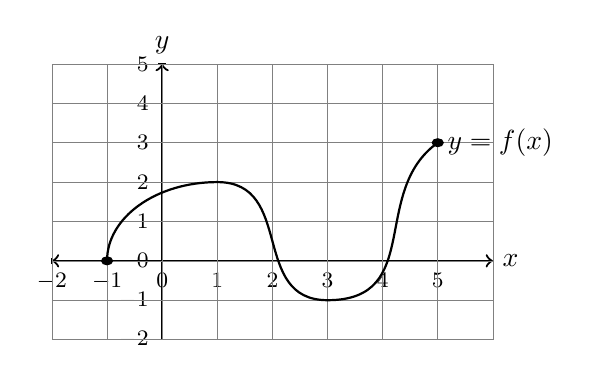
\begin{tikzpicture}[xscale=.7,yscale=.5]
\foreach \x in {-2,-1,0,1,2,3,4,5}\draw[shift={(\x,0)},color=black] (0pt,2pt) -- (0pt,-2pt) node[below] {\footnotesize $\x$};
\foreach \y in {-2,-1,0,1,2,3,4,5}\draw[shift={(0,\y)},color=black] (2pt,0pt) -- (-2pt,0pt) node[left] {\footnotesize $\y$};
\draw[thick] [<->] (-2,0) -- (6,0);
\draw[thick] [->] (0,-2) -- (0,5);
\draw [help lines] (-2,-2) grid (6,5);
\node[align=center,right] at (6,0){$x$};
\node[align=center,above] at (0,5){$y$};
\node[align=center,right] at (5,3){$y=f(x)$};
\draw [fill] (-1,0) circle [radius=0.1];
\draw [fill] (5,3) circle [radius=0.1];
\draw[thick] (-1,0) to [out=90,in=180] (1,2)
to [out=0,in=180] (3,-1) to [out=0,in=225] (5,3) ;
\end{tikzpicture} 
\end{figure}

If we build a new function $y = f(x) + a$, where $a$ is a positive number, each output is increased by $a$. Hence, because of addition being represented as upward motion, the graph is shifted up by $a$ units. Likewise, if the new function is $y = f(x)-a$, the graph is shifted down by $a$ units (remember, we assumed $a$ was positive). In the following figure, we have the graph of $f$ along with its vertical shifts by $1$ and $-1$.

\begin{figure}[h]
\centering
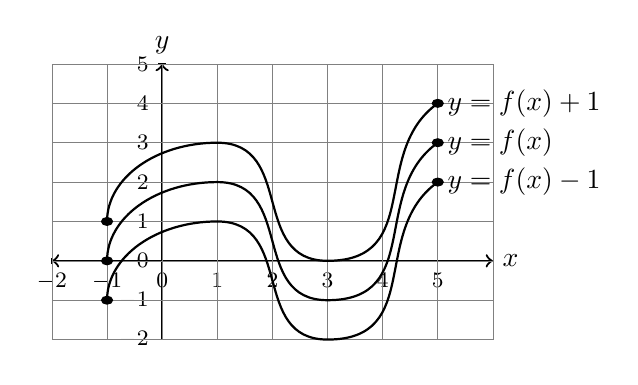
\begin{tikzpicture}[xscale=.7,yscale=.5]
\foreach \x in {-2,-1,0,1,2,3,4,5}\draw[shift={(\x,0)},color=black] (0pt,2pt) -- (0pt,-2pt) node[below] {\footnotesize $\x$};
\foreach \y in {-2,-1,0,1,2,3,4,5}\draw[shift={(0,\y)},color=black] (2pt,0pt) -- (-2pt,0pt) node[left] {\footnotesize $\y$};
\draw[thick] [<->] (-2,0) -- (6,0);
\draw[thick] [->] (0,-2) -- (0,5);
\draw [help lines] (-2,-2) grid (6,5);
\node[align=center,right] at (6,0){$x$};
\node[align=center,above] at (0,5){$y$};
\node[align=center,right] at (5,3){$y=f(x)$};
\node[align=center,right] at (5,4){$y=f(x)+1$};
\node[align=center,right] at (5,2){$y=f(x)-1$};
\draw [fill] (-1,0) circle [radius=0.1];
\draw [fill] (5,3) circle [radius=0.1];
\draw[thick] (-1,0) to [out=90,in=180] (1,2)
to [out=0,in=180] (3,-1) to [out=0,in=225] (5,3) ;

\draw [fill] (-1,1) circle [radius=0.1];
\draw [fill] (5,4) circle [radius=0.1];
\draw[thick] (-1,1) to [out=90,in=180] (1,3)
to [out=0,in=180] (3,0) to [out=0,in=225] (5,4) ;

\draw [fill] (-1,-1) circle [radius=0.1];
\draw [fill] (5,2) circle [radius=0.1];
\draw[thick] (-1,-1) to [out=90,in=180] (1,1)
to [out=0,in=180] (3,-2) to [out=0,in=225] (5,2) ;
\end{tikzpicture} 
\caption{Vertical shifts of magnitude one.}
\end{figure}

\begin{question} Let $f(x) = 3(0.5)^x$. What is the range of $f$? What is the range of $f(x) + a$ when $a$ is any number (not necessarily just positive)? Explain.
\end{question}

\par

Now we will move on to the effect of multiplication on the outside of a function. Suppose our parent function is $y=f(x)$ and $k>1$, then $y = kf(x)$ has a graph that is that of $f$, except stretched away from the $x$-axis by a factor of $k$. this is due to the geometric representation of multiplication by numbers greater than one being represented as a stretch away from zero. Likewise, if $0<k<1$, then the graph is compressed vertically by a factor of $k$. If $k$ is negative, then the graph is first reflected across the $x$-axis, then stretched or compressed by the magnitude of $k$. This is due to our representation of multiplication by negative numbers as reflection, followed by a stretch or compression.   

\begin{figure}[h]
\centering
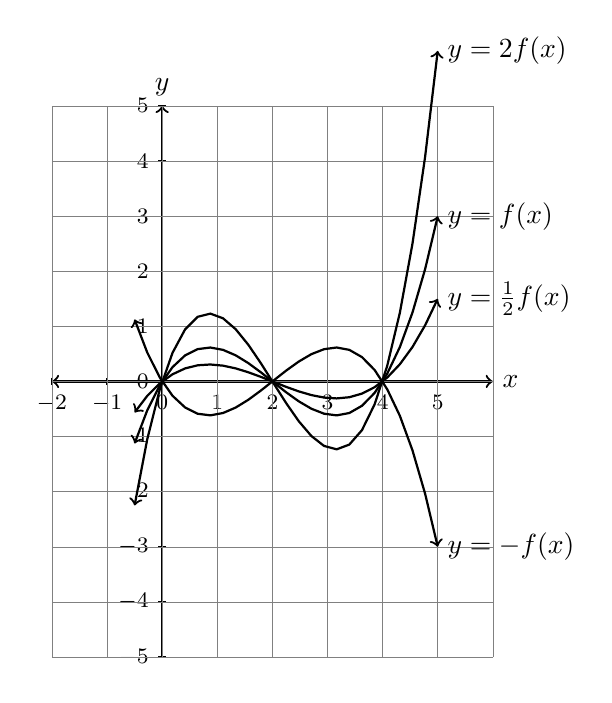
\begin{tikzpicture}[xscale=.7,yscale=.7]
\foreach \x in {-2,-1,0,1,2,3,4,5}\draw[shift={(\x,0)},color=black] (0pt,2pt) -- (0pt,-2pt) node[below] {\footnotesize $\x$};
\foreach \y in {-5,-4,-3,-2,-1,0,1,2,3,4,5}\draw[shift={(0,\y)},color=black] (2pt,0pt) -- (-2pt,0pt) node[left] {\footnotesize $\y$};
\draw[thick] [<->] (-2,0) -- (6,0);
\draw[thick] [->] (0,-5) -- (0,5);
\draw [help lines] (-2,-5) grid (6,5);
\node[align=center,right] at (6,0){$x$};
\node[align=center,above] at (0,5){$y$};
\node[align=center,right] at (5,3){$y=f(x)$};
\node[align=center,right] at (5,-3){$y=-f(x)$};
\node[align=center,right] at (5,6){$y=2f(x)$};
\node[align=center,right] at (5,1.5){$y=\frac{1}{2}f(x)$};
\draw [thick,domain=-.5:5] [<->] plot (\x, {0.2*(\x - 2)*(\x)*(\x-4)});
\draw [thick,domain=-.5:5] [<->] plot (\x, {0.4*(\x - 2)*(\x)*(\x-4)});
\draw [thick,domain=-.5:5] [<->] plot (\x, {0.1*(\x - 2)*(\x)*(\x-4)});
\draw [thick,domain=-.5:5] [<->] plot (\x, {-0.2*(\x - 2)*(\x)*(\x-4)});
\end{tikzpicture} 
\caption{A vertical stretch, a compression, and a reflection.}
\end{figure}

\begin{question} Suppose $f$ has a horizontal intercept at $x=r$. Symbolically, this means $f(r) = 0$. What happens to the location of this intercept when the function is transformed into $kf(x)$? Explain both graphically and symbolically.
\end{question}

\par

\begin{question} Describe what happens to the $y$-intercept of a function under the action of each of the basic outside transformations.
\end{question}

\par

Now we will describe the effect of inside transformations. First, consider adding a positive number $a$ to $x$, before $f$ is applied. Because $a$ is added to $x$ before $f$ is applied, the output of $f(x+a)$, for any given $x$, will be equal to the output of $f(x)$ at a point $a$ units to the right of $x$. Hence, we have the following:
\\
\begin{center}
The graph of $f(x+a)$ is the graph of $f(x)$, except shifted $a$ units to the left.\\
\end{center}
Likewise, the graph of $f(x-a)$ is that of $f(x)$, except shifted to the right by $a$ units.

\par

This may seem counter intuitive at first, because adding should move things to the right. However, finding an $x$-value for a given $y$-value will involve solving for $x$, which means the last step we will do is subtract, i.e. move to the left. For instance, consider the following example:

\par 

\begin{eg} Let $f(x) = \sqrt{x-3} + 5$. One simple point on the graph of this function is $(4,6)$, because $f(4) = \sqrt{4-3} + 5 = 6$. Now let's consider the new function $g(x) = f(x+2) = \sqrt{(x+2)-3} + 5$. To find the transformed version of $(4,6)$ on the graph of $g$, we must solve:
\begin{eqnarray*}
\sqrt{(x+2) - 3} + 5 & = & 6\\
& \updownarrow & \\
(x+2) - 3 & = & 1\\
& \updownarrow & \\
(x+2) & = & 4\\
& \updownarrow & \\
x = 2.
\end{eqnarray*}
Thus the transformed point is $(2,6)$, which is two units to the left of $(4,6)$.\qed \end{eg}

\begin{figure}[h]
\centering
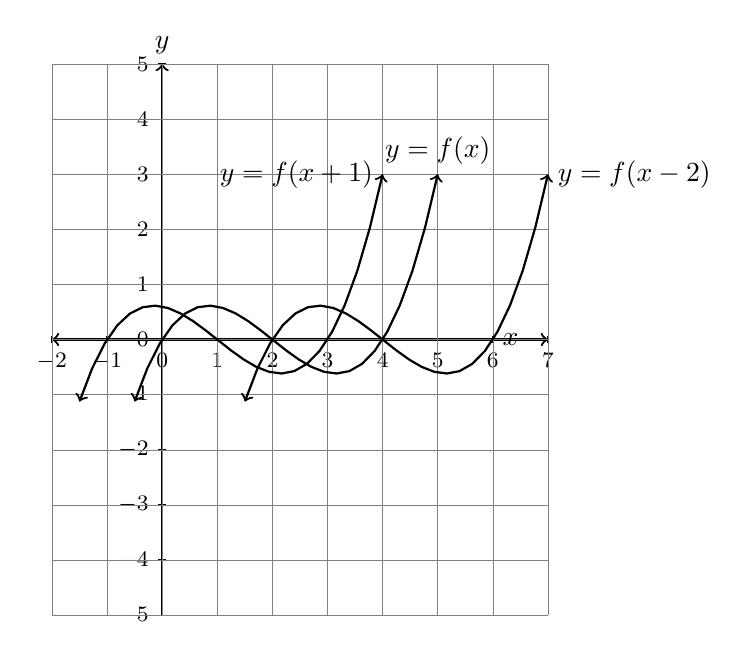
\begin{tikzpicture}[xscale=.7,yscale=.7]
\foreach \x in {-2,-1,0,1,2,3,4,5,6,7}\draw[shift={(\x,0)},color=black] (0pt,2pt) -- (0pt,-2pt) node[below] {\footnotesize $\x$};
\foreach \y in {-5,-4,-3,-2,-1,0,1,2,3,4,5}\draw[shift={(0,\y)},color=black] (2pt,0pt) -- (-2pt,0pt) node[left] {\footnotesize $\y$};
\draw[thick] [<->] (-2,0) -- (7,0);
\draw[thick] [->] (0,-5) -- (0,5);
\draw [help lines] (-2,-5) grid (7,5);
\node[align=center,right] at (6,0){$x$};
\node[align=center,above] at (0,5){$y$};
\node[align=center,above] at (5,3){$y=f(x)$};
\node[align=center,right] at (7,3){$y=f(x-2)$};
\node[align=center,left] at (4,3){$y=f(x+1)$};

\draw [thick,domain=-.5:5] [<->] plot (\x, {0.2*(\x - 2)*(\x)*(\x-4)});
\draw [thick,domain=1.5:7] [<->] plot (\x, {0.2*(\x - 4)*(\x-2)*(\x-6)});
\draw [thick,domain=-1.5:4] [<->] plot (\x, {0.2*(\x - 1)*(\x+1)*(\x-3)});
\end{tikzpicture} 
\caption{Left and right shifts.}
\end{figure}

\par

\begin{question} Let $f(x) = \frac{1}{(x+4)(x-5)}$. What is the domain of $f(x)$? What is the domain of $f(x-a)$, where $a$ is a real number?
\end{question}

\par 

Multiplication as an inside transformation is handled similarly to addition. Suppose $f$ is a parent function, and we want to see the effect of multiplying $x$ by some constant $k$, before $f$ is applied. If $k>1$, then for any given $x$, the output of $f(kx)$ will be that of $f(x)$ at a point that is a factor of $k$ further away from the $y$-axis. Thus, when $k>1$, we have
\\
\begin{center}
The graph of $f(kx)$ is the graph of $f(x)$, except compressed by a factor of $\frac{1}{k}$ toward the $y$-axis.\\
\end{center}
Likewise, the graph of $f(kx)$ is that of $f(x)$, except stretched away from the $y$-axis by a factor of $\frac{1}{k}$ when $0<k<1$ (so $\frac{1}{k} > 1$). If $k$ is negative, the graph of $f(kx)$ is first reflected over the $y$-axis, then compressed or stretched according to the absolute value of $k$.

\begin{figure}[h]
\centering
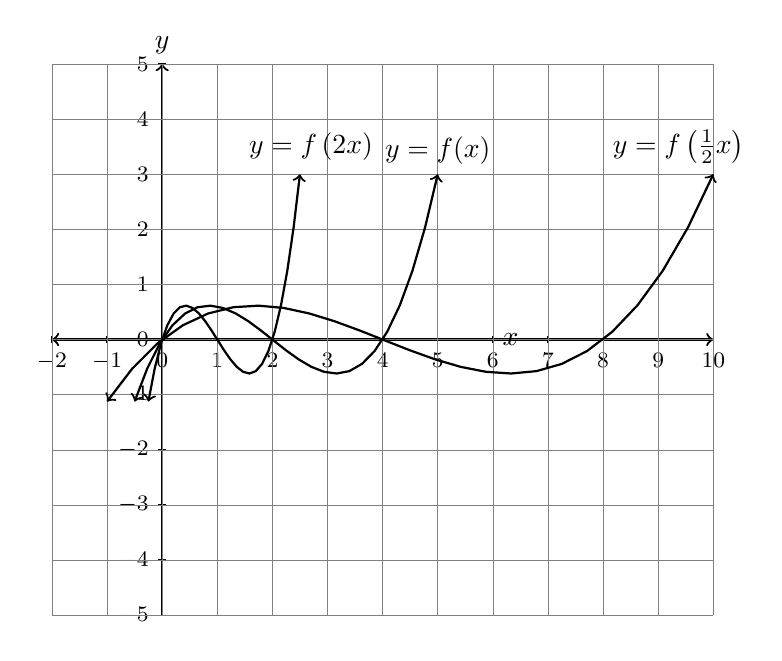
\begin{tikzpicture}[xscale=.7,yscale=.7]
\foreach \x in {-2,-1,0,1,2,3,4,5,6,7,8,9,10}\draw[shift={(\x,0)},color=black] (0pt,2pt) -- (0pt,-2pt) node[below] {\footnotesize $\x$};
\foreach \y in {-5,-4,-3,-2,-1,0,1,2,3,4,5}\draw[shift={(0,\y)},color=black] (2pt,0pt) -- (-2pt,0pt) node[left] {\footnotesize $\y$};
\draw[thick] [<->] (-2,0) -- (10,0);
\draw[thick] [->] (0,-5) -- (0,5);
\draw [help lines] (-2,-5) grid (10,5);
\node[align=center,right] at (6,0){$x$};
\node[align=center,above] at (0,5){$y$};
\node[align=center,above] at (5,3){$y=f(x)$};
\node[align=center,right] at (8,3.5){$y=f\left(\frac{1}{2}x\right)$};
\node[align=center,left] at (4,3.5){$y=f\left(2x\right)$};

\draw [thick,domain=-.5:5] [<->] plot (\x, {0.2*(\x - 2)*(\x)*(\x-4)});
\draw [thick,domain=-.25:2.5] [<->] plot (\x, {0.2*(2*\x - 2)*(2*\x)*(2*\x-4)});
\draw [thick,domain=-1:10] [<->] plot (\x, {0.2*(.5*\x - 2)*(.5*\x)*(.5*\x-4)});
\end{tikzpicture} 
\caption{A horizontal stretch and compression.}
\end{figure}

\par

\begin{question} Suppose $(2,3)$ is on the graph of $y=f(x)$, that is $f(2) = 3$. What point is on the graph of $y = f(-2x) + 1$? Explain both graphically and symbolically.
\end{question}


\subsection{Function Families and Graphical Transformations}

Some of our important forms for certain function families may be thought of as graphical transformations of some building block members of the given family.

\begin{eg} Consider the basic linear function with slope $m$, $y = f(x) = mx$. The $y$-intercept of this function is at $(0,0)$. In order to obtain a new linear function whose graph passes through the point $(x_0,y_0)$, we can perform a horizontal shift to the right by $x_0$ units and a vertical shift up by $y_0$ units to obtain
\[
y = f(x-x_0) + y_0 = m(x-x_0) + y_0.
\]
This is simply the point-slope form for a line with slope $m$ passing through the point $(x_0,y_0)$.\qed \end{eg}

\begin{eg} Consider a basic quadratic function $f(x) = ax^2$, where $a$ is some given number. The vertex of its graph is at $(0,0)$. In order to have the vertex occur at $(h,k)$, we simply shift it to get
\[
 y = f(x-h)+k = a(x-h)^2 + k.
\]
This is the vertex form of a quadratic.\qed \end{eg}

\par

\begin{question} Use factored form to find the formula for a quadratic function $f(x)$ whose $x$-intercepts are at $(1,0)$ and $(4,0)$, and whose $y$-intercept is at $(0,7)$. What does the parameter $a$ (which you must solve for) do graphically?
\end{question}


\begin{question} In building an exponential function, $Q = f(t)$, with an initial value of five that grows by $3\%$ for each ten unit increase in $t$, we find
\[
Q = f(t) = 5(1.03)^{t/10}.
\]
Explain how this function can be built using two graphical transformations of $g(t) = (1.03)^t$.
\end{question} 

\vfill  
